\section{Introducción}
\label{sec:intro}

En la presente sección se intentará explicar brevemente el contexto actual del desarrollo
de software y las motivaciones del presente trabajo, así como del lenguaje de programación
elegido para el desarrollo.\\
Se comenzará por un análisis sobre la evolución de las tecnologías actuales y como estas
han derivado a la generación de aplicaciones hechas mayormente en \htmlv. Luego se enumeraran
los distintos factores que inciden sobre la elección del lenguaje de programación a
utilizar, mostrando como los lenguajes para la \jvm son una buena elección debido a su
popularidad y a la compatibilidad de código entre lenguajes que corren sobre la
plataforma. Finalmente se explicará la estructura básica de las aplicaciones web desarrolladas
sobre lenguajes de la \jvm, y como se manejan las \dependencies en estas aplicaciones.\\

\subsection{Sobre los sistemas web}
\label{subsec:intro:about_web}

Si bien no es el objetivo de este documento explicar en detalle la historia de los cambios
en las arquitecturas de software, este apartado intentará dar una breve muestra de las
transformaciones que ha sufrido la industria de desarrollo de sistemas en los últimos
tiempos, y como estas han llevado a que los sistemas web sean hoy en día una de las
opciones más utilizadas en el ámbito empresarial.

\subsubsection{Estado anterior a los sistemas web}
\label{subsubsec:intro:about_web:previous_pc}

En las décadas de 1960 y 1970, comienza en el mundo un proceso lento pero incremental de
computarización de la información. Las computadoras dejan de ser \quoted{juguetes}
científicos para pasar a ser complejas maquinarias con verdadera utilidad practica
en distintas industrias.\\
Durante esos años varias empresas comienzan a \emph{informatizarse}. Bancos, petroleras
y otros, compran grandes computadoras capaces de almacenar toda su información o procesar
complejos cálculos matemáticos en poco tiempo.\\
En este contexto, múltiples empresas como \emph{IBM}, \emph{RCA}, y 
\emph{General Electric}, comenzaron a fabricar gigantescas computadoras de precio cada
vez más económico. Estas maquinas evolucionarían poco a poco hasta convertirse en lo que
hoy se conocen como \mainframes.\\
En este sentido, \citefullauthor{Stephens:2008:BOOK} en su libro
\citetitle{Stephens:2008:BOOK} \citeyearsq{Stephens:2008:BOOK} describe a un \mainframe
como una computadora muy grande, con una base de datos de alto rendimiento, a la cual se
accede desde una terminal remota, es decir, una maquina \quoted{tonta}, sin mucha otra
finalidad más que la de conectarse al servidor central para realizar peticiones de datos
y mostrarle los resultados al usuario.\\
\citeauthor{Stephens:2008:BOOK} también destaca los beneficios de los \mainframes por
sobre una computadora personal a nivel empresarial. Las características que menciona son:
\begin{description}
	\item[Integridad de datos:] Los datos \textsc{deben} ser correctos.
	\item[Rendimiento:] Se debe procesar gran cantidad de datos.
	\item[Respuesta:] El procesamiento debe ser inmediato.
	\item[Recuperación ante desastres:] En caso de un fallo, se debe volver a estar
	operativo inmediatamente.
	\item[Usabilidad:] Debe hacer lo que se requiere, cuando se requiere.
	\item[Confiabilidad:] No debe fallar y siempre debe estar disponible.
	\item[Auditoria:] Ser capaz de saber quien realizó qué acción en el equipo.
	\item[Seguridad:] Solo aquellos que pueden realizar una acción pueden hacerlo.
\end{description}
Estas características son todavía buscadas en los grandes \mainframes de la actualidad,
y resultan fundamentales en emprendimientos críticos, por ejemplo, sistemas bancarios,
programas de control de acciones financieras, sistemas petroleros o el software que
controla misiones espaciales.\\
\citefullauthor{Elliot:2008:BOOK} ha descripto que las tendencias de la
tecnología utilizada, no obedecen solamente a motivaciones económicas y operativas, sino
a un complejo entramado de relaciones entre empresas que comparten una visión utópica
sobre la tecnología en cuestión \citesq[pag 3]{Elliot:2008:BOOK}. Así, las empresas
comercializadoras de \mainframes enarbolando como bandera principal los beneficios
planteados por \citeauthor{Stephens:2008:BOOK}, lograron generar una visión utópica en
las empresas usuarias para posicionar la tecnología dominante durante largos años.
Es por esto que los \mainframes siguen teniendo hoy en día un lugar en el mercado.\\
 
\subsubsection{Aparición de las computadoras personales}
\label{subsubsec:intro:about_web:pc_era}

A partir de fines de los 70`s y comienzos de los 80`s, las \acp{pc}
comienzan a ser cada vez más accesibles \citesq[cap 4]{Allan:2001:BOOK}.
La liberación de \emph{ARPANET} por parte de \acs{darpa} en 1983 da nacimiento
a \internet. Estos dos cambios suponen un quiebre en las tecnologías de uso
empresarial.\\
El \ac{pc}, sumado a la conectividad y nuevas tecnologías tanto en sistemas como en
lenguajes de programación llevaron a que los \mainframes comenzaran a perder terreno.\\
La posibilidad de ejecutar programas en cada \ac{pc} dio lugar a nuevas arquitecturas
\clientserver. Ahora los usuarios corrían los programas en su propio equipo, permitiendo
aumentar la velocidad de respuesta. El programa se conectaba a \internet y sincronizaba
información con un servidor central solo cuando fuera necesario.\\
Esta arquitectura permitiría una más rápida evolución del software por sobre la opción de
tener el sistema en un \mainframe, como explican \citefullauthor{Duncan:1996:ARTICLE}
en su artículo \citetitle{Duncan:1996:ARTICLE}\period Sin embargo, como contrapartida  estos
cambios suponen un alto costo de mantenimiento, y en caso de poseer equipos con distintos
sistemas operativos, un gasto extra en el desarrollo. Esto se debe a la necesidad de
generar un cliente para cada sistema operativo, y la necesidad de actualizar los mismos
en caso de futuros cambios\footnote{
	Recuerde el lector que el software se distribuía en esa época en medios físicos, por
	lo que la instalación de una nueva versión del sistema requería presencia física en el
	equipo.
}.
Así, los autores demuestran que, independientemente de los costos, el factor más incidente
en el cambio es la necesidad de mantener el sistema al día con las necesidades de la empresa.

\subsubsection{Navegadores y primeros sistemas web}
\label{subsubsec:intro:about_web:web}

Tras la aparición de los navegadores web, como \emph{Netscape} e \emph{Internet Explorer},
a comienzos de 1990, se comenzaron a desarrollar los primeros sistemas web.\\
Los mismos, consistían básicamente en documentos dinámicos, generados con información
tomada de una base de datos. Gran influencia tuvieron en este tipo de soluciones, la
creación de lenguajes de programación y tecnologías pensadas para generar documentos
\gls{html} dinámicamente \citesq[pag 2]{Hunter:2001:BOOK}, como \emph{PHP}, \emph{ASP}
y los \emph{Servlets} de \java.
La posibilidad de generar \emph{aplicaciones} que corran en el navegador, solucionó las
problemáticas asociadas a el mantenimiento de los sistemas y al desarrollo para múltiples
sistemas operativos. Sin embargo, esta vez, la naturaleza de \html limitaba la capacidad
de las aplicaciones a sencillos formularios, botones y enlaces.\\
Estas limitaciones hicieron que no fuera sino hasta con la aparición de las primeras
tecnologías complementarias a \html, que las aplicaciones web comenzarían a cobrar
relevancia, dando lugar a las \ac{ria}.

\subsubsection{Rich Internet Applications}
\label{subsubsec:intro:about_web:rias}

Las \glspl{ria} surgen para compensar aquellas faltantes que
presentaban las aplicaciones web frente a las tradicionales de \clientserver de
escritorio.\\
En un primer lugar, software en forma de complementos (\plugins) que permitían correr
algún lenguaje especial en los navegadores
fueron creados. Uno de los más populares fue \emph{Flash} de \emph{Adobe}, que continua
siendo utilizado hoy en día. \java tampoco se quedo atrás y presentó sus \servlets,
una forma de embeber código Java en páginas \html.\\
Las \ria comenzaron a copar los mercados empresariales, ya que permitían ahorrar
en mantenimiento y desarrollo, a la vez que brindaban la alta usabilidad que se demandaba
de un sistema empresarial.\\
Cada vez más soluciones comenzaron a surgir, \emph{Adobe Flex},
\emph{Microsoft Silverlight} y \emph{JavaFX} \citesq{Clarke:2009:BOOK}. Sin embargo, la
falta de estándares llevaría a que se desarrollaran con fuerza \gls{css} y
\gls{js}, tecnologías libres y disponibles en cualquier navegador sin necesidad de
instalar software adicional.\\
Así, en los últimos años,y gracias también al auge de los smartphones y tablets, incapaces
de correr los anteriormente mencionados \plugins, el llamado \gls{html5}
pasaría a transformarse en el estándar para el desarrollo de \rias
\citesq{David:2013:BOOK}.\\
La tendencia marca que las \rias desarrolladas bajo el estándar \htmlv seguirán siendo la
norma durante los años venideros. Múltiples \frameworks han aparecido capaces de generar
rápidamente sistemas web con una interfaz completamente realizado en \htmlv.\\



\subsection{Acerca de la Java Virtual Machine (\jvm)}
\label{subsec:intro:about_jvm}

Con la popularidad de \java, comenzaron a surgir una serie de lenguajes que compilan a
\bytecode para la \acl{jvm}. Estos lenguajes se presentan como alternativas para los
programadores de la plataforma que buscan una opción "superior", en algún aspecto,
a \java. \groovy por ejemplo, se presenta como un lenguaje dinámico, similar a Ruby;
\clojure es una extensión de Lisp apuntado a la Programación Concurrente; \scala es un
lenguaje que presenta características tanto de Programación Funcional como de
Programación Orientada a Objectos. También existen otra numerosa cantidad de lenguajes,
algunos experimentales, algunos con una base creciente de usuarios, que corren sobre la
plataforma, como también una amplia cantidad de adaptaciones de lenguajes populares para
que corran en la \jvm, como JRuby y Jython, versiones de Ruby y Python que compilan a
\bytecode java.\\
Una característica interesante de estos lenguajes es que el código compilado suele ser
compatible entre si, es decir, código escrito en \java puede ser ejecutado en \scala,
codigo \groovy puede ser usado desde \clojure, etc.\footnote{
	Si bien mayoritariamente esto es cierto, ciertas caracteristicas especiales de algunos
	lenguajes no pueden ser empleadas desde otros, presentando así ciertas limitaciones de
	compatibilidad. Sin embargo, se espera que futuras versiones de la \jvm permitan un
	grado de compartición de código entre lenguajes aún mayor.
}.\\
Finalmente, podemos destacar el hecho de que hoy en día existen numerosas implementaciones
de la \jvm, tanto propietarias como libres, muchas con fines muy específicos, como Dalvik,
la \jvm del sistema operativo Android \citesq{Wikipedia:2012:ONLINE}.\\


\subsection{Crecimiento de la \jvm como plataforma}
\label{subsec:intro:jvm_growth}

\java es, casi sin cuestionamientos \footnote{
	Se puede argumentar que la medición de la popularidad de
	los lenguajes de programación es una ciencia inexacta, pues los factores de medición no
	se encuentran determinados. Sumado a esto, la mayoría de los resultados se basa en
	cantidad de lineas de código y menciones online, hecho que no tiene en consideración las
	diferencias entre un lenguaje y otro, ya que algunos son necesariamente más
	verborragicos que otros (Por ejemplo, dos códigos que realizan exactamente la misma
	acción en dos lenguajes distintos pueden resultar en cantidades significativamente
	distintas de lineas de código entre uno y otro, solo por la sintaxis y la naturaleza
	misma del lenguaje.) Así, cada estadista toma distintas variables, le otorga distinto
	peso a las mismas y obtendrá distintos resultados.
}, uno de los lenguajes más populares. Así lo demuestran las estadísticas de análisis de
popularidad de lenguajes, como la renombrada estadística TIOBE que a la fecha de esta
publicación ubica a \java en segundo lugar [\citefullauthor{TIOBE:2014:ONLINE},
\citeyear{TIOBE:2014:ONLINE}]. La estadística \emph{"transparente"} creada por
\citefullauthor{Montmollin:2013:ONLINE}, que publica el código de forma open source y
sus reglas online, muestra al lenguaje de Oracle en la misma posición
\citesq{Montmollin:2013:ONLINE}, mientras que la otra herramienta open source que
permite medir la popularidad de los lenguajes, PyPL, de
\citefullauthor{Carbonelle:2014:ONLINE}, lo muestra en primer lugar
\citesq{Carbonelle:2014:ONLINE}.\\
Además, \citefullauthor{Kunst:2014:ONLINE} ha desarrollado un gráfico en donde muestra la
cantidad de líneas de código en \gls{github} por sobre las menciones en
\gls{stackoverflow}, mostrando a \java por sobre los más populares, pero también a los
lenguajes que corren sobre la \jvm\footnote{
	Entre los lenguajes para la \jvm se encuentran \scala, \clojure, \groovy, AspectJ,
	Ceylon, Fantom, Fortress, Frege, Gosu, Ioke, Jelly, Kotlin, Mirah, Processing, X10,
	Xtend, Rhino, JRuby, Jython, entre otros. Aunque no todos se encuentran mencionados
	en la gráfica.
} como de alto interés.\\
Queda entonces patente que los lenguajes que se ejecutan en la \jvm tienen un uso cada vez
mayor. Empero, la diferencia se volvería aún más grande si se considera el uso de los
lenguajes para desarrollo de soluciones web.\\
Si bien no existen estadísticas que confirmen esto, es prácticamente reconocido por
cualquier programador que la ventaja que se lee en las estadísticas por parte del lenguaje
C, es producto del desarrollo, no de sistemas web, sino de pequeñas herramientas de
escritorio. Asimismo, la popularidad creciente de Objective-C, se debe al uso del mismo en
las aplicaciones móviles de iPhone y iPad. Finalmente, el amplio desarrollo que presenta
en las encuestas \js, no compite necesariamente con los sistemas hechos en \jvm sino que
de hecho, tiende a complementarlos, ya que es una parte importante de las
\rias\see{subsubsec:intro:about_web:rias}.\\



\subsection{Desarrollo de sistemas web en la \jvm}
\label{subsec:intro:jvm_dev}

Al desarrollar sistemas web se puede elegir cualquiera de los lenguajes para
la \jvm, y dentro del mismo, cualquiera de los numerosos \frameworks que trabajan
con \htmlv existentes. Sin embargo hay ciertas constantes comunes de todos los
lenguajes y \frameworks antes mencionados. A continuación se analizaran estos
componentes comunes para comprender la forma de desarrollar en los mismos.

\subsubsection{Estructura común de sistemas web}
\label{susubbsec:intro:jvm_dev:structure}

La mayoría de los sistemas web suelen dividirse en capas (También llamadas
\emph{layers} o \emph{tiers}). Estas capas suelen dividirse de forma tal que
cada una esté encargada de partes muy puntuales de la lógica de la aplicación.\\
La mayoría de los autores  suelen identificar tres capas, las cuales, dependiendo
del autor, suelen recibir distintos nombres. Sin embargo, la estructura es siempre
la misma. Estas capas son: la de interfaz o \view, la de \logic,
modelo o aplicación y la de \data o persistencia.\\
La capa de datos es la encargada de manejar los accesos a la base de datos, persistir
la información, y todo lo relacionado a elementos de los que se deba guardar registro.
La capa de lógica de negocios es la que contiene el código de las competencias de la
aplicación, es decir, las cosas que la aplicación puede hacer, su funcionalidad.
Finalmente, la capa de interfaz es la que permite acceder a la funcionalidad y visualizar
los datos a los usuarios o clientes \citesq[pag 29-30]{Barish:2002:BOOK}.
La \figref{fig:intro:jvm:web_arch} muestra la arquitectura básica de una aplicación
web según este esquema.\\
En los últimos años, el crecimiento de las tecnologías móviles han hecho que la
arquitectura cambie a una más orientada a servicios, donde el servidor no genera
documentos que serán procesados por el usuario, sino que este, consumirá solamente
datos expuestos por el servidor, encargándose el cliente de la parte de la interfaz.
De esta forma, un mismo sistema web puede ser utilizado para mostrar una página en un
navegador, o por una aplicación para teléfonos móviles\citesq{MacVittie:2008:ONLINE}.
La \figref{fig:intro:jvm:new_web_arch} muestra la arquitectura con este nuevo
paradigma.

\begin{figure}[t]
	\centering
	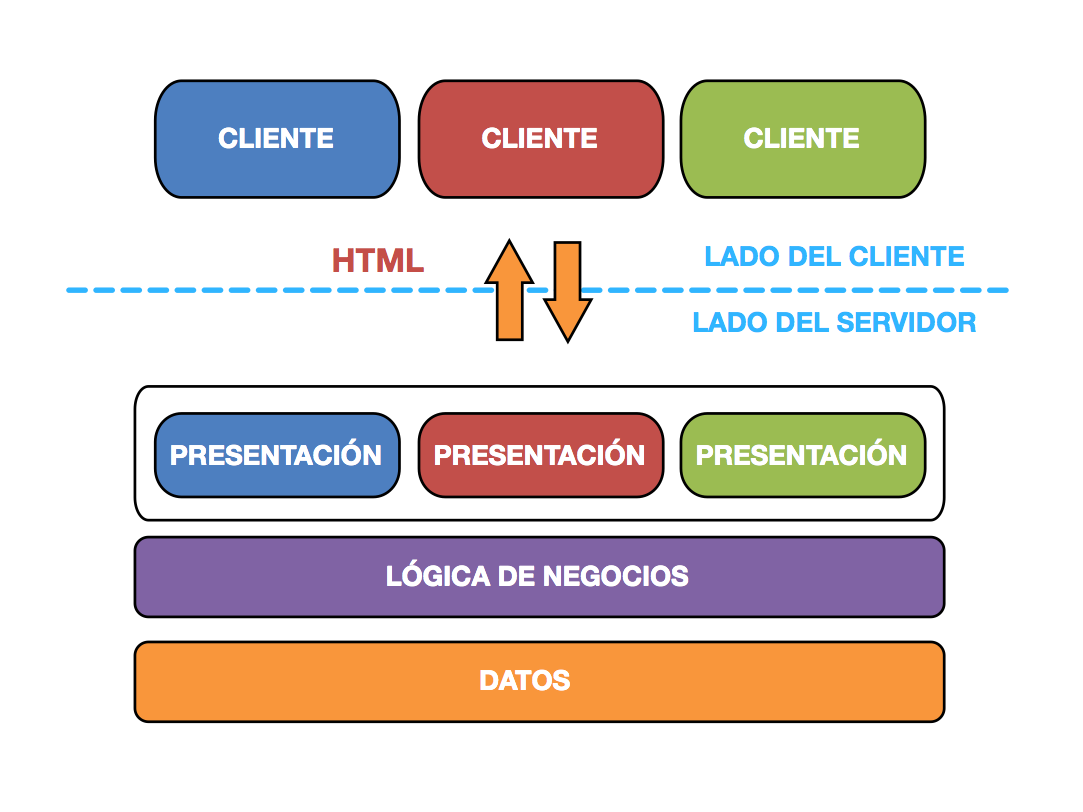
\includegraphics[]{figures/web_arch.png}
	\caption{Arquitectura em capas básica de un sistema web.}
	\label{fig:intro:jvm:web_arch}
\end{figure}

\begin{figure}[t]
	\centering
	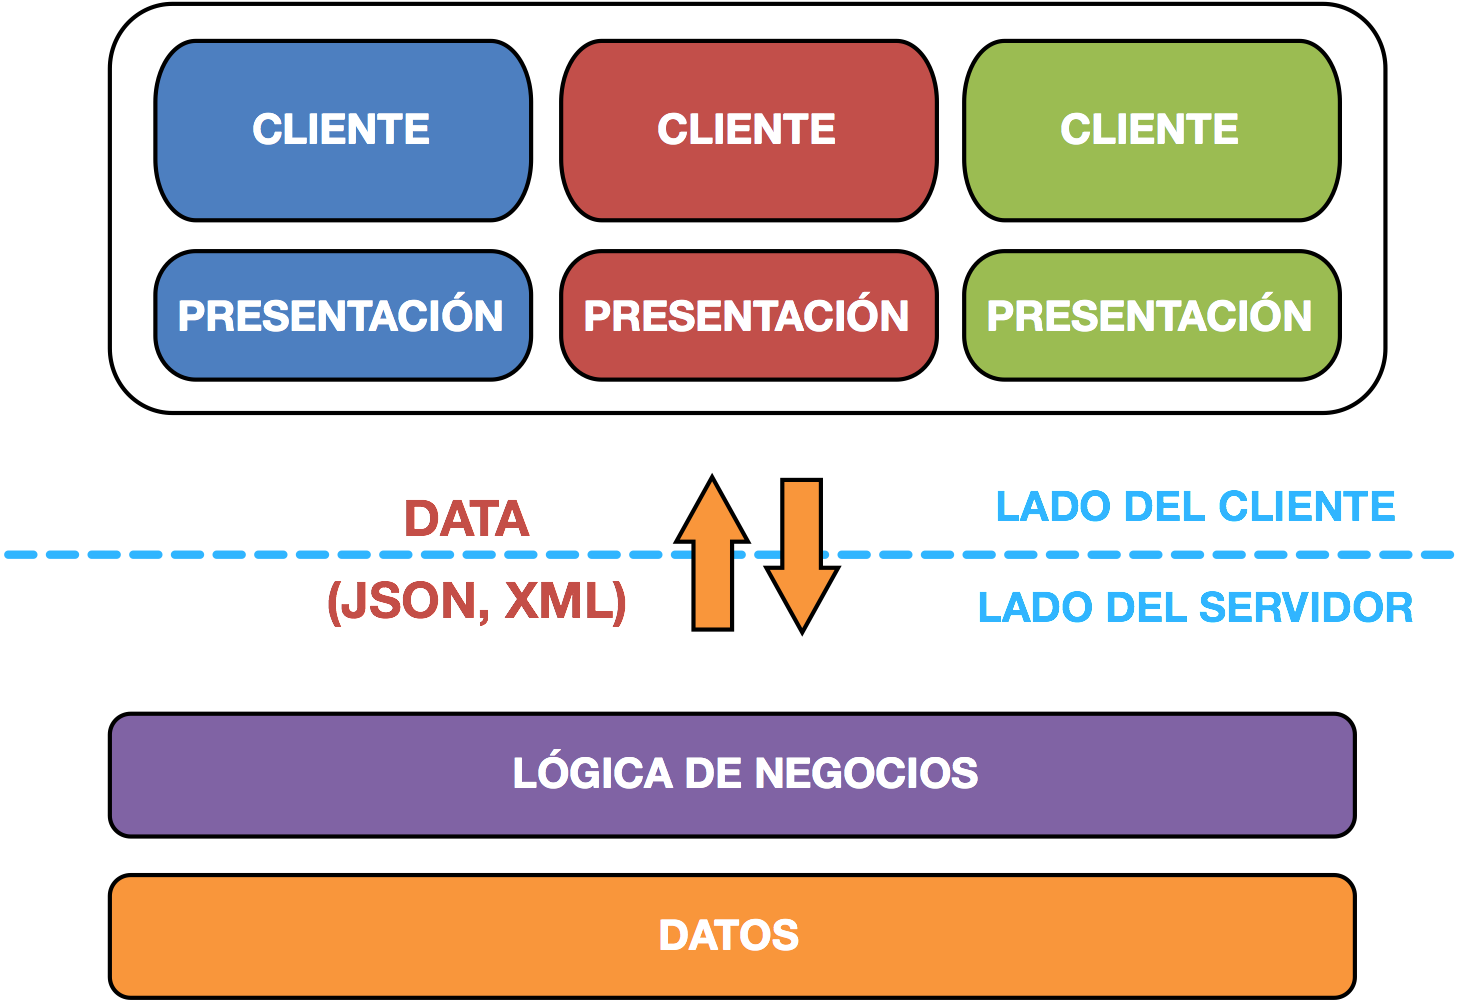
\includegraphics[]{figures/new_web_arch.png}
	\caption{Arquitectura em capas de los nuevos sistemas web.}
	\label{fig:intro:jvm:new_web_arch}
\end{figure}

 
\subsubsection{Reutilización de código mediante dependencias}
\label{susubbsec:intro:jvm_dev:dependencies}

Prácticamente ningún desarrollador comienza una aplicación completamente desde
cero, haciendo a la conocida frase \quoted{Pararse sobre hombros de gigantes} una
constante en el desarrollo de software, en especial en el empresarial. Así, existen
numerosos \frameworks, \toolkits, bibliotecas, y porciones de código que los
desarrolladores pueden importar en el propio, de forma de obtener funcionalidades
genéricas previamente desarrolladas.\\
Estas porciones de código de terceros que utilizan los desarrolladores en sus
proyectos recibe el nombre de \dependencies. Las mismas son necesarias
para que un proyecto funcione correctamente.\\
Se pueden distinguir dos tipos de \dependencies, las manejadas y las no manejadas.
Las \dependencies no manejadas son código que se agrega manualmente al
proyecto mediante la clásica técnica de \quoted{copiar y pegar} o agregando los archivos
correspondientes a esa \dependency en alguna carpeta del proyecto (Proceso al que
se denominará \quoted{instalar}). Por su parte, las manejadas, consisten en algún tipo de
descripción en un archivo de configuración o símil que identificará a las \dependencies
requeridas. Un programa externo evaluara nuestro archivo de configuración y se encargará
de instalar nuestras \dependencies declaradas, estos programas son conocidos como
\depmgrs.\\
Las \dependencies no manejadas suelen implicar una serie de pasos repetitivos y propensos
a errores que el usuario debe realizar con el objetivo de poder correr su código. Por su
parte, las \dependencies manejadas son preferentes, ya que eliminan errores comunes y
ahorran tiempo y trabajo a los desarrolladores. Además, los \depmgrs
suelen ahorrar el trabajo que implica instalar las \dependencies anidadas\footnote{
	Asuma el lector un proyecto \emph{A} con una \dependency \emph{B}. El paquete \emph{B}
	es a su vez un proyecto con \dependencies, por ejemplo \emph{C}. Para que \emph{A}
	funcione correctamente, requiere \emph{B} y este a su vez requiere \emph{C}, haciendo
	que de forma transitiva \emph{A} requiera \emph{C}.
} \citesq{Larman:2010:BOOK}.\\
Finalmente, en este escrito, se identificaran dos tipos más de dependencias. las de la
\logictier, dadas por \emph{paquetes} de código \java compilado (archivos .jar o .war),
y las de \viewtier que consisten en, pero no se limitan a, archivos \css y \js.\\
En las subsecciones siguientes se verá como estas dependencias son abordadas por los
desarrolladores que trabajan en lenguajes de la \jvm en la actualidad.

\subsubsection{Dependencias manejadas de la \logictier}
\label{susubbsec:intro:jvm_dev:logic_dependencies}

El desarrollo en la plataforma \java se volvió muy popular rápidamente, y por tanto,
un gran numero de herramientas surgieron para asistir al desarrollador al momento
de programar.\\
En el ámbito del manejo de \dependencies en la \logictier la herramienta \emph{Maven}
de la fundación \emph{Apache} se ha posicionado como el estándar de facto\footnote{
	Si bien \emph{Apache Maven} es en realidad no solo un \depmgr
	sino un administrador de proyectos, provee la funcionalidad antes mencionada y
	la misma se ha vuelto un estándar.
} \citesq{Sonatype:2008:BOOK}. Otro de los proyectos que se han posicionado en esta área
es \emph{Apache Ivy}, que se concentra solamente en el manejo de \dependencies.\\
Maven hace uso de un archivo de configuración escrito en \gls{xml}\footnote{
	Este archivo es comunmente denominado POM, ya que el nombre del archivo debe ser
	pom.xml.
}. El \coderef{code:intro:jvm:maven_pom}
muestra un ejemplo de este tipo de archivo de configuración.
\\
\begin{pomcode}[caption=Configuración de \dependencies en Maven mediante archivo POM,
	label=code:intro:jvm:maven_pom]
<project>
	...
	<dependencies>
		<dependency>
			<groupId>group-a</groupId>
			<artifactId>artifact-a</artifactId>
			<version>1.0</version>
		</dependency>
		<dependency>
			<groupId>group-a</groupId>
			<artifactId>artifact-b</artifactId>
			<version>1.0</version>
		</dependency>
	</dependencies>
</project>
\end{pomcode}

Ivy utiliza también archivos \xml, pero estos son más compactos que los de Maven.
El \coderef{code:intro:jvm:ivy_module} es un ejemplo del mismo.
\\
\begin{ivycode}[caption=Archivo de configuración de Ivy,
	label=code:intro:jvm:ivy_modulue]
<ivy-module version="2.0">
	<info organisation="org.apache" module="hello-ivy"/>
	<dependencies>
		<dependency org="group-a" name="artifact-a" rev="1.0"/>
		<dependency org="group-b" name="artifact-b" rev="1.0"/>
	</dependencies>
</ivy-module>
\end{ivycode}

Con la aparición de nuevos lenguajes para la \jvm comenzaron a surgir nuevos
\depmgrs, como Grape o Gradle para Groovy, \sbt para Scala y
Leiningen para Clojure, y Apache Buildr como propuesta multilenguaje. Cada uno
de ellos utilizan un archivo de configuración con
distinta sintaxis \citesq[pág. 569]{Alexander:2013:BOOK}. El
\coderef{code:intro:jvm:sbt_module_add} muestra un ejemplo de
la declaración de una \dependency en el archivo de configuración de \sbt.
\\
\begin{javacode}[caption=Dependencia de SpringFramework 3.1.1 para \sbt,
	label=code:intro:jvm:sbt_module_add]
libraryDependencies += "org.springframework.data" %  "spring-data-neo4j" %  "3.1.1.RELEASE"
\end{javacode}

A pesar de este hecho, todos los \depmgrs trabajan bajo el
estándar pre-impuesto por Maven, siendo así al punto tal de que el sitio
\gls{mvnrepo} es el centro de referencia al momento de buscar dependencias.

\subsubsection{Dependencias no manejadas de \viewtier}
\label{susubbsec:intro:jvm_dev:view_dependencies}

Lamentablemente, la falta de estándares para desarrollar \rias en la \viewtier 
durante largos años
llevó a que no hayan herramientas sencillas para instalar \dependencies que
corran en la misma. La mayoría de estas \dependencies consisten en archivos
\css y \js, los cuales suelen ser descargados manualmente a través de la
página del creador del código (No existen repositorios centralizados como
en el caso de las \dependencies de la \logictier). Luego, los archivos deben
ser copiados a alguna carpeta del proyecto (la ubicación exacta depende de
la estructura del proyecto y por tanto debe ser recordada por el programador)
para encontrarse finalmente disponibles para su importación y uso en el código
del usuario.\\
Si bien el proceso parece sencillo, las aplicaciones web se han vuelto cada
vez más y más complejas. Las posibilidades que brindan los navegadores aumentan
y, por tanto, también aumentan las \dependencies ya que se requieren cada vez
cosas más especificas\footnote{
	Un claro ejemplo de esto son las \gls{webfonts}. Las mismas
	no comenzaron a ser comunes sino hasta hace unos pocos años, y hoy en día
	son usadas en enorme cantidad de sitios.
}.\\
A su vez, los tipos de \dependency son más variados (No son solo archivos jar o war),
dando por resultado un catálogo mucho más amplio, donde una misma \dependency no
necesariamente consiste en un único archivo, sino en múltiples archivos de distinto
formato que deben ser agregados al proyecto de una forma especifica. La falta de un
lugar que agrupe
estos contenidos y estandarice sus nombres, versiones, formas de instalación, etc. hace que sea muy
difícil manejar estas \dependencies.

\subsubsection{CDN}
\label{susubbsec:intro:jvm_dev:cdns}

Las \cdn surgen con la idea de agrupar el contenido disponible\footnote{
	Su creación no responde necesariamente a procesos de manejo de dependencias
	en proyectos de desarrollo de software, sin embargo es uno de los usos
	posibles de este tipo de redes y ha sido uno de los usos más comunes.
}.\\
Las \gls{cdn} permiten al usuario insertar en su codigo HTML una clausula que
importa automáticamente la dependencia requerida desde el servidor más cercano.
\\
\begin{htmlcode}[caption=Dependencias agregadas mediante \cdn,
	label=code:intro:cdn:cdn_deps]
<html>
	<head>
		...
		<!-- JQuery -->
		<script src="//ajax.googleapis.com/ajax/libs/jquery/1.11.1/jquery.min.js"></script>
		<!-- JQuery Mobile -->
		<link rel="stylesheet" href="//ajax.googleapis.com/ajax/libs/jquerymobile/1.4.3/jquery.mobile.min.css" />
		<script src="//ajax.googleapis.com/ajax/libs/jquerymobile/1.4.3/jquery.mobile.min.js"></script>
		<!-- JQuery UI -->
		<link rel="stylesheet" href="//ajax.googleapis.com/ajax/libs/jqueryui/1.11.0/themes/smoothness/jquery-ui.css" />
		<script src="//ajax.googleapis.com/ajax/libs/jqueryui/1.11.0/jquery-ui.min.js"></script>
	</head>
	<body>
		...
	</body>
</html>
\end{htmlcode}

El \coderef{code:intro:cdn:cdn_deps} utiliza la \cdn de \citeauthor{GoogleCDN:ONLINE}
(\citeurl{GoogleCDN:ONLINE}) una de las más populares y confiables junto con la de
\citeauthor{MicrosoftCDN:ONLINE} (\citeurl{MicrosoftCDN:ONLINE}) y los sitios
\citeurl{jsDelivrCDN:ONLINE} y \citeurl{CDNjs:ONLINE}.\\
Las \cdns no solo brindan el beneficio de facilitar el manejo de dependencias,
sino que a su vez le ahorra trabajo a los servidores de nuestra aplicación, que no
requiere servir algunos archivos, y puede, en teoría, ser beneficioso
para los usuarios, ya que el servidor de la \cdn podría estar más cerca de su área que
el de la aplicación, facilitando la carga del sitio.\\
Como contrapartida, las \cdns suelen tener una gestión centralizada, con lo cual es
difícil contar con las ultimas versiones, o con bibliotecas que los administradores
del mismo decidan no colocar. Así, muchas bibliotecas y \frameworks no se encuentran
disponibles en las \cdns más populares. A esto se le agrega el alto costo de mantener
una \cdn por cualquier empresa que no posea grandes servidores a lo largo del globo.

\subsubsection{Dependencias manejadas de \viewtier}
\label{susubbsec:intro:jvm_dev:view_managed}

Surgió entonces la necesidad de contar con \depmgrs para
la \viewtier y que no requiera de la disponibilidad de terceros como las \cdns.
Así surgieron soluciones que manejan las \dependencies de forma similar a la
forma en que lo hacen los manejadores de la \logictier.\\
\emph{Bower} y \emph{Component} \footnote{
	Component es más similar a Maven ya que se encarga de muchas
	otras cosas además del manejo de dependencias, como procesos de compilación.
}, son casi con seguridad, los más populares de estos sistemas. Ambos son modulo de
la plataforma \gls{node} y poseen formas de manejar las \dependencies mediante un
archivo de configuración. Sin embargo, ambas requieren en la mayoría de los casos
contar con herramientas externas como git, ya que se desentienden del proceso de
mantenimiento de repositorios \cite{Bower:ONLINE}.\\
\emph{RequireJS} y \emph{Browserify} son otras soluciones que manejan las dependencias
\js solamente y no utilizan la técnica de archivos de configuración
\citesq{Franko:2013:BOOK}.\\
Todas estas soluciones se presentan bastante incompletas en comparación a las
disponibles en la \viewtier. Además, al requerir herramientas que no son
independientes del sistema operativo, generan muchas complicaciones al momento
de configurar el entorno de desarrollo o de puesta en producción del sistema.
Como si esto no fuera suficiente, el desarrollador debe aprender una nueva
tecnología, proceso que lleva tiempo y esfuerzo del que a veces no dispone.